% !TEX TS-program = pdflatex
\documentclass[aps,prc,twocolumn,floatfix,showpacs,preprintnumbers,amsmath,amssymb,superscriptaddress,linenumbers]{revtex4-1}
\usepackage{hyperref}
\usepackage{latexsym}
\usepackage{verbatim}
\usepackage{graphics}
\usepackage{caption}
\usepackage{subfigure}
\usepackage{amsmath}
\captionsetup{justification=centerlast,font=small,margin=0.5cm}
\usepackage{setspace}
\usepackage{graphicx,amsmath,color}% Include figure files
\usepackage[normalem]{ulem} %for strikeouts
\usepackage{todonotes}
\usepackage{placeins}


\providecommand{\Journal}[4] {#1 {\bf #2}, #3 (#4)}
\providecommand{\EPJC}{Eur. Phys. J. C }
\providecommand{\NCA}{Nuovo Cimento }
\providecommand{\NIM}{Nucl. Instr. Methods }
\providecommand{\NIMA}{Nucl. Instr. Meth. A }
\providecommand{\NPA}{Nucl. Phys. A }
\providecommand{\NPB}{Nucl. Phys. B }
\providecommand{\NHPA}{Nucl. Hadr. Phys. A }
\providecommand{\PLB}{Phys. Lett. B }
\providecommand{\PR}{Phys. Rev. }
\providecommand{\PRL}{Phys. Rev. Lett. }
\providecommand{\PRC}{Phys. Rev. C }
\providecommand{\PRD}{Phys. Rev. D }
\providecommand{\RMP}{Rev. Mod. Phys. }
\providecommand{\ZPC}{Z. Phys. C }
\providecommand{\qqb}{$q\bar{q}$~}
\newcommand{\bff}{{}}

\definecolor{lightred}{rgb}{1,0.5,0.5}
\definecolor{lightgreen}{rgb}{0.5,1,0.5}
\definecolor{darkgreen}{rgb}{0.5,0.9,0.5}

\def\piz{\pi^{0}}
\def\pizT{$\pi^{0} \ $}
\def\epemT{$ e^+e^-  $}
\def\epem{e^+e^-}

\definecolor{Mycolor2}{HTML}{0c9008}

\begin{document}


%----------------------------------------------------
\begin{figure*}[htb!]
\centerline{
	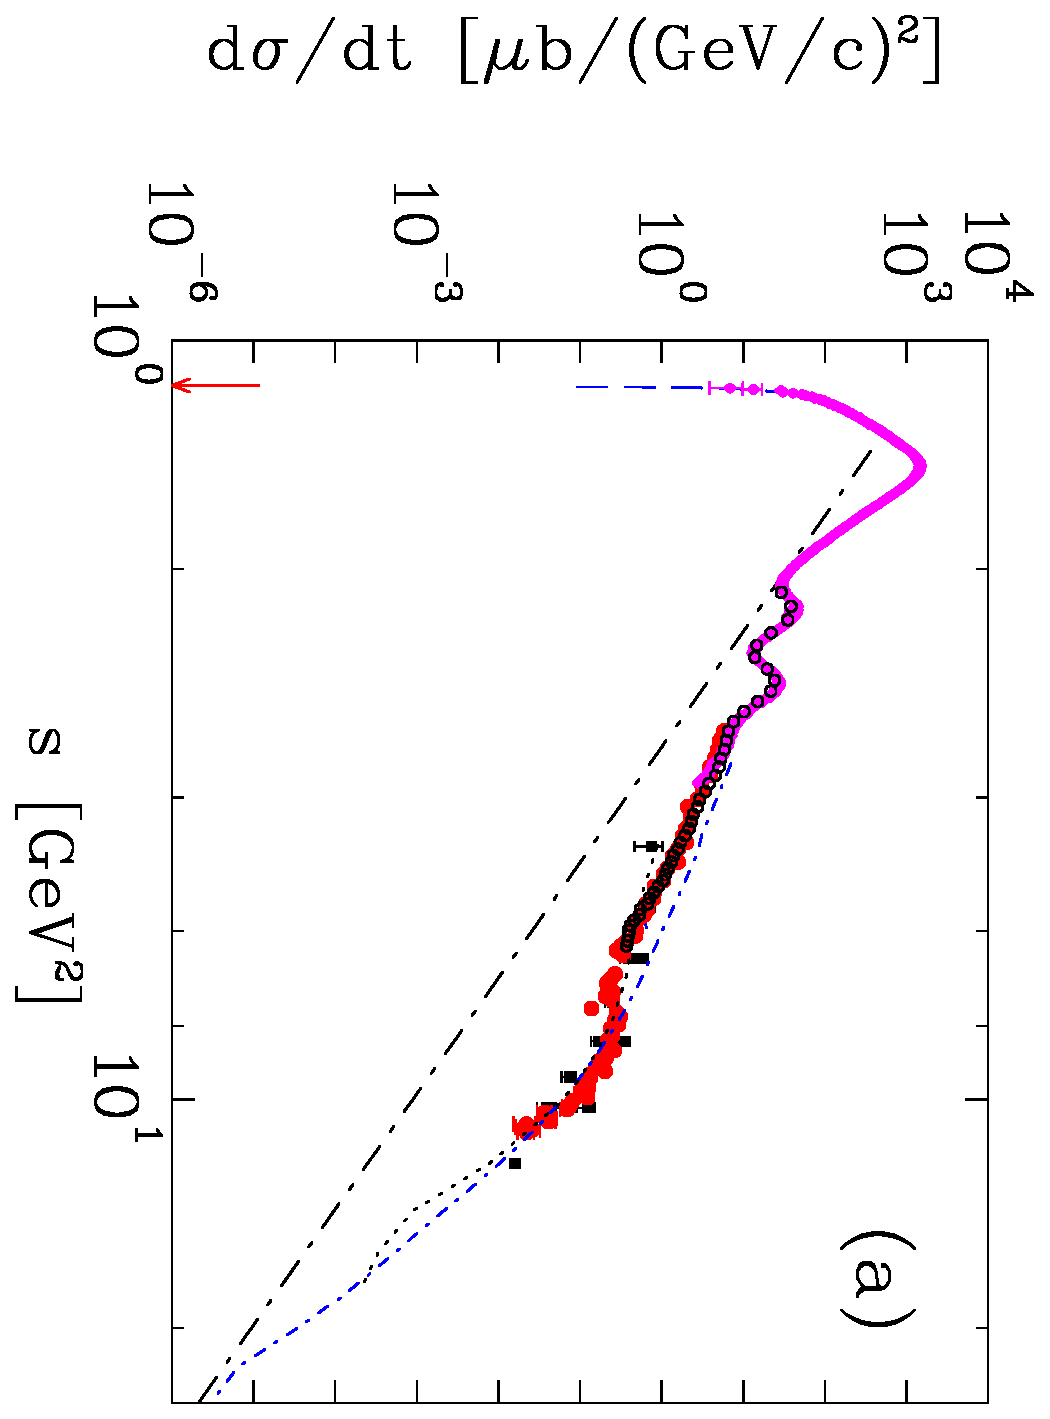
\includegraphics[height=0.4\textwidth, angle=90]{scale50.eps}\hfill%\hspace{1.5cm}
	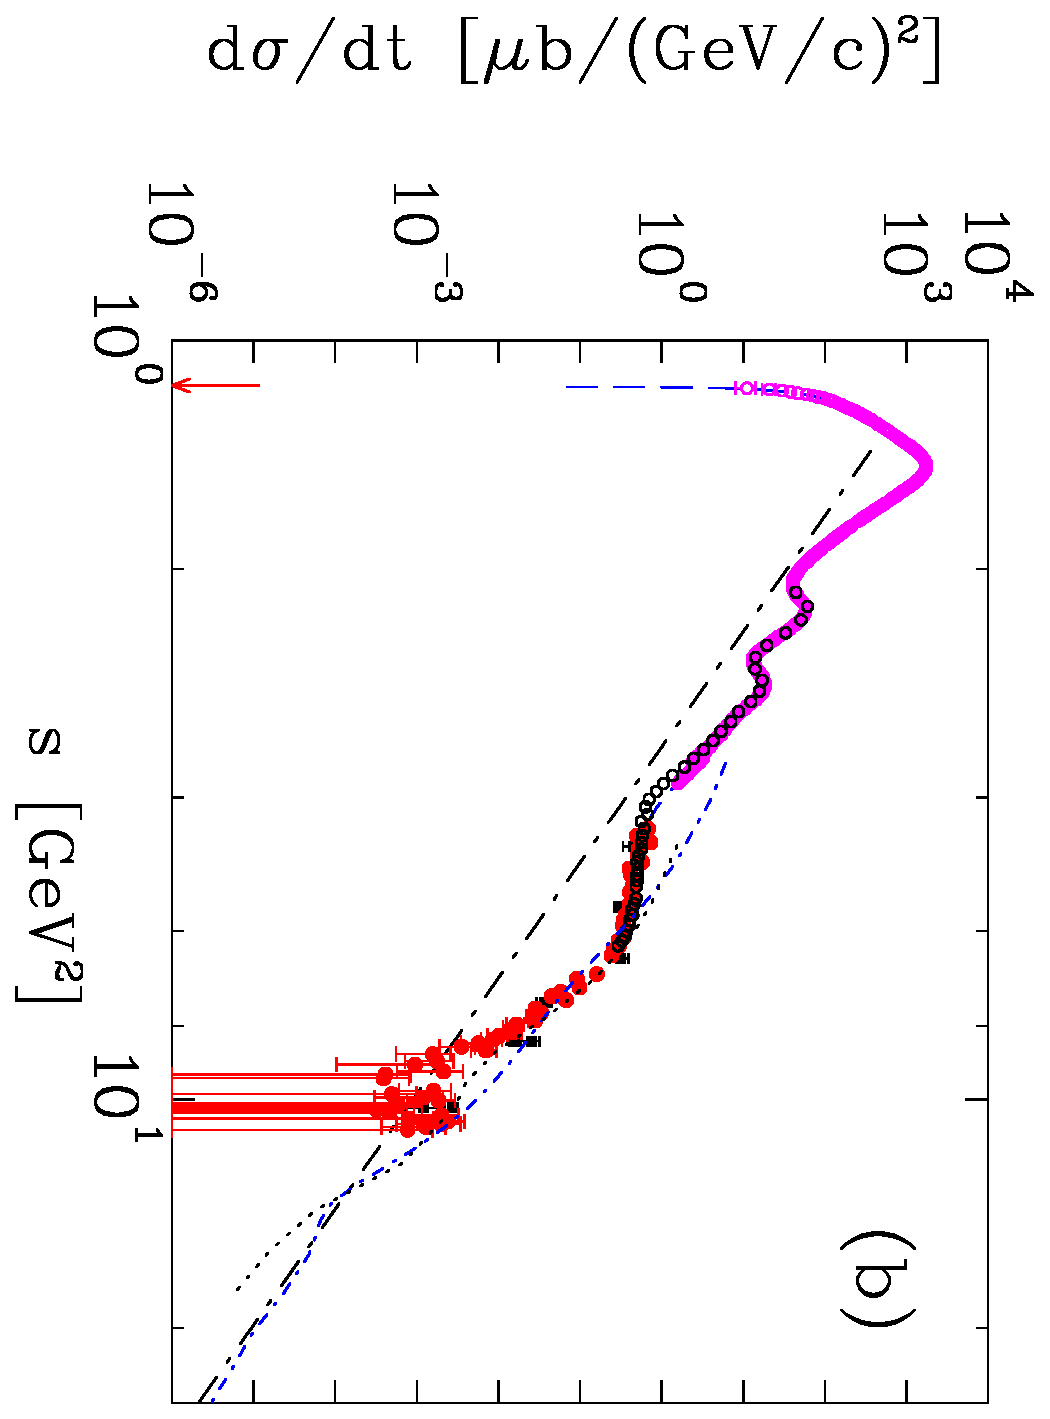
\includegraphics[height=0.4\textwidth, angle=90]{scale70.eps}}
\centerline{
        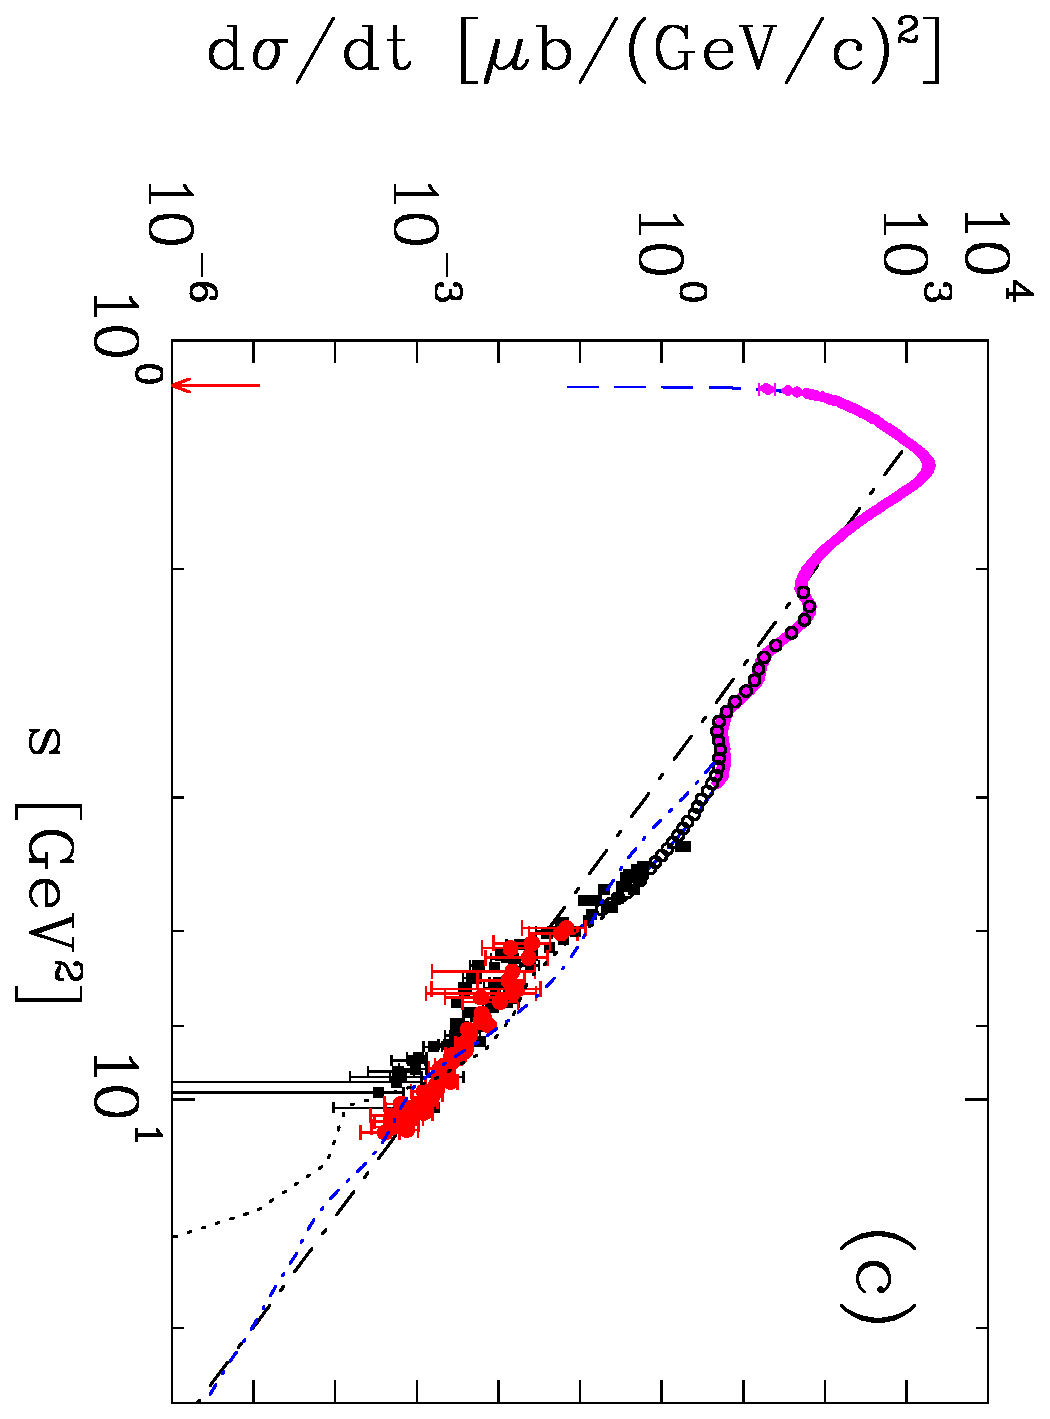
\includegraphics[height=0.4\textwidth, angle=90]{scale90.eps}\hfill%\hspace{1.5cm}
        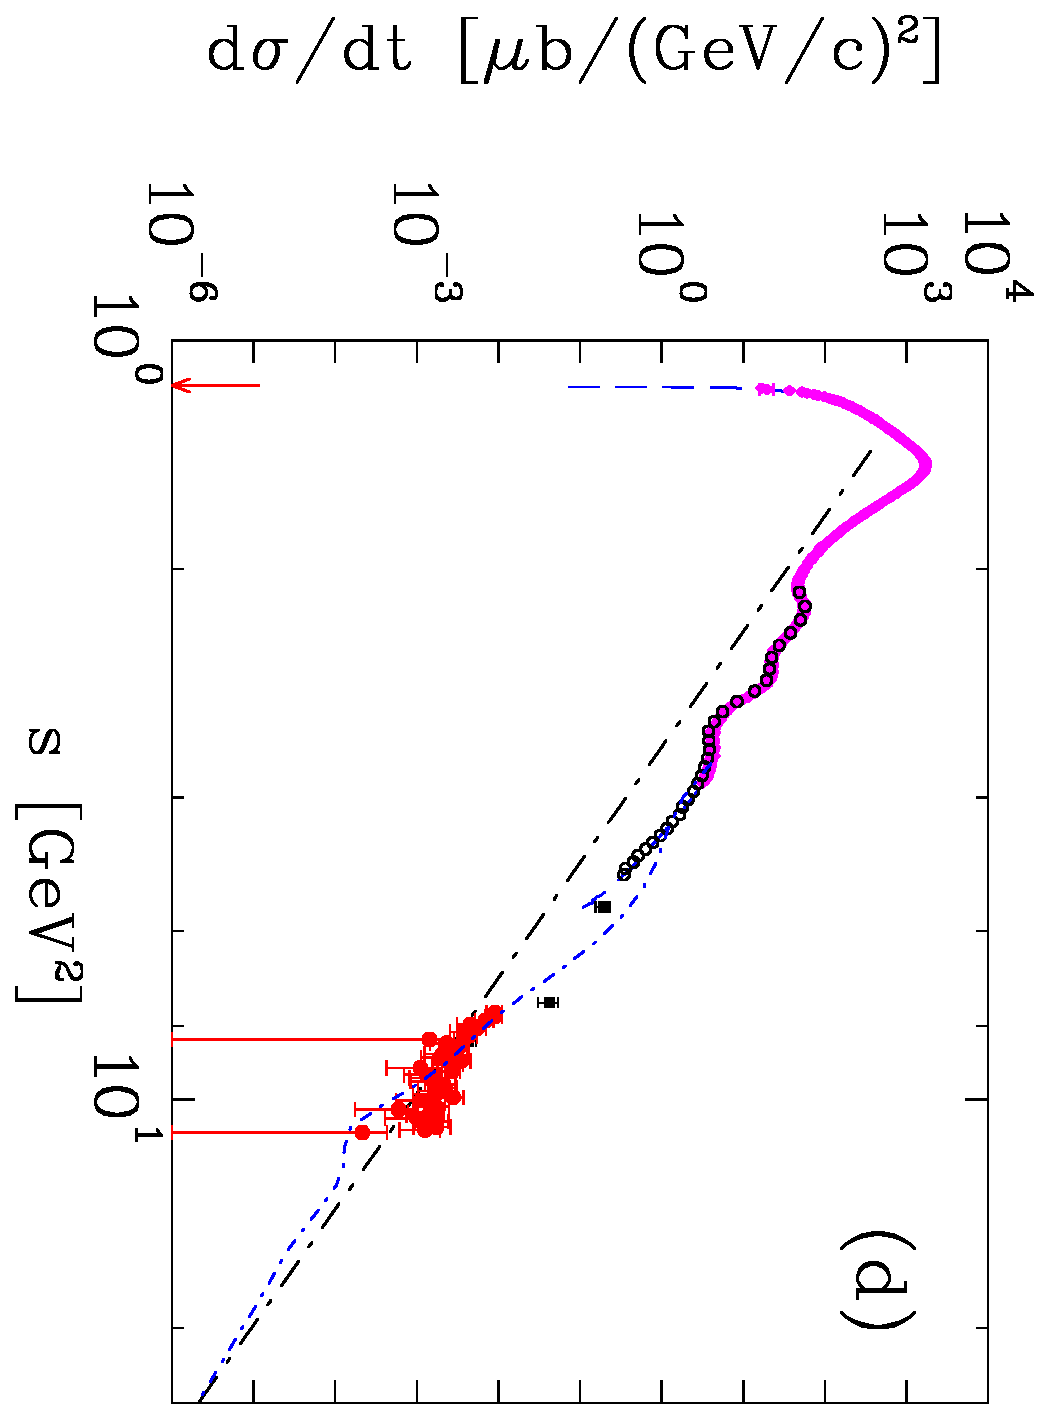
\includegraphics[height=0.4\textwidth, angle=90]{scale110.eps}}

        \caption {EPStoPDF} \label{fig:scaling}
\end{figure*}

\begin{figure*}[htb!]
\centerline{
	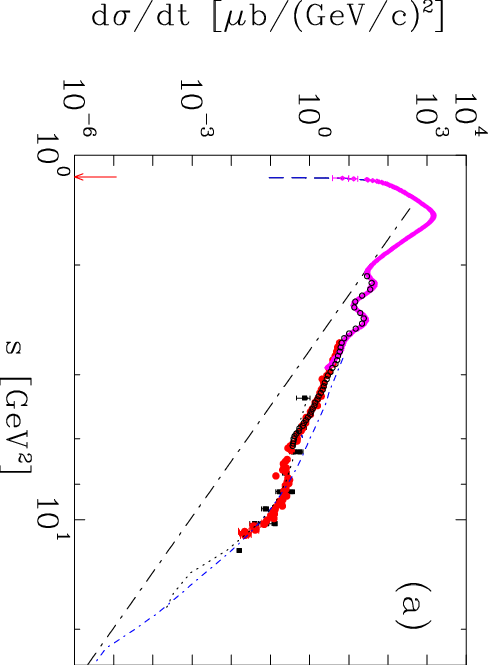
\includegraphics[height=0.4\textwidth, angle=90]{scale50.png}\hfill%\hspace{1.5cm}
	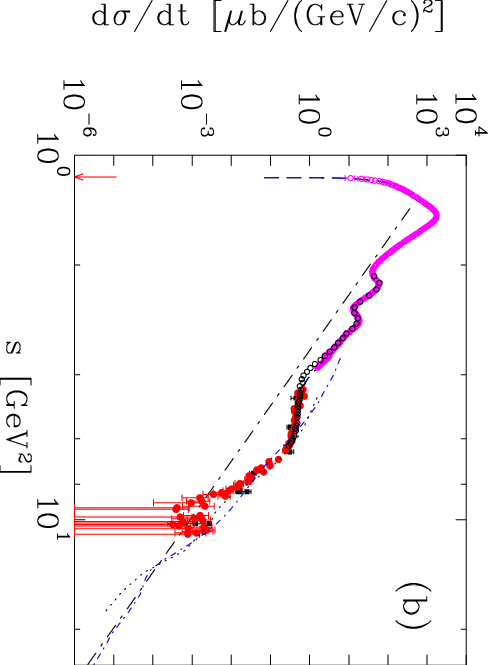
\includegraphics[height=0.4\textwidth, angle=90]{scale70.png}}
\centerline{
        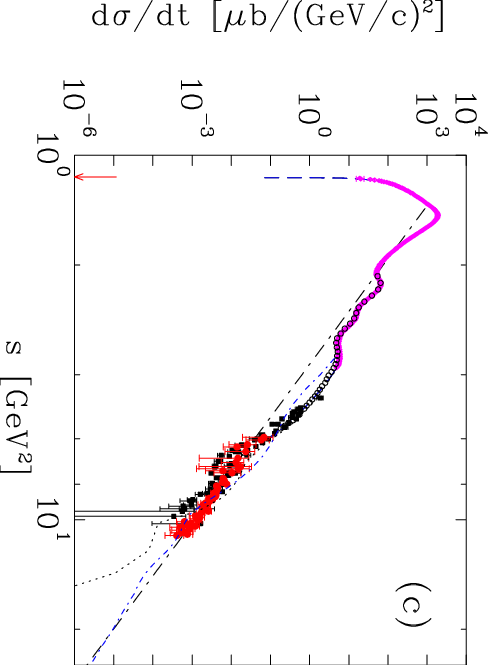
\includegraphics[height=0.4\textwidth, angle=90]{scale90.png}\hfill%\hspace{1.5cm}
        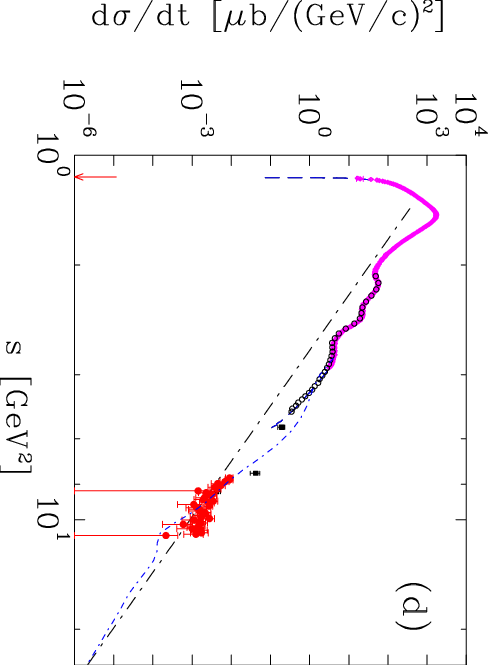
\includegraphics[height=0.4\textwidth, angle=90]{scale110.png}}

        \caption {PNG} \label{fig:scalingPNG}
\end{figure*}
%-----------------------------------------------------


\begin{figure*}[htb!]
\centerline{
        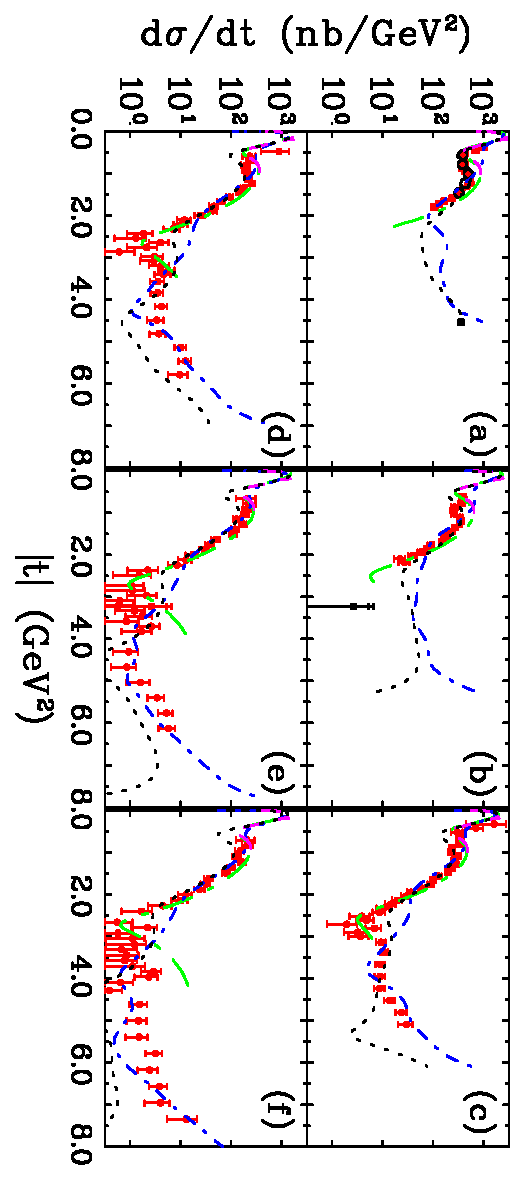
\includegraphics[width=3in, angle=90]{dsdt.eps}}

        \caption {EPStoPDF} 
	\label{fig:t_data}
\end{figure*}
\begin{figure*}[htb!]
\centerline{
        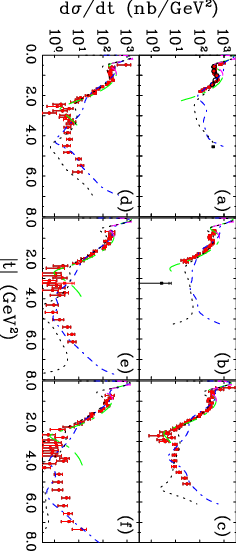
\includegraphics[width=3in, angle=90]{dsdt.png}}

        \caption {PNG} 
	\label{fig:t_dataPNG}
\end{figure*}
%-----------------------------------------------------

%------------------------------------------------------
%\begin{figure}[htb!]
\begin{figure}
\centerline{
        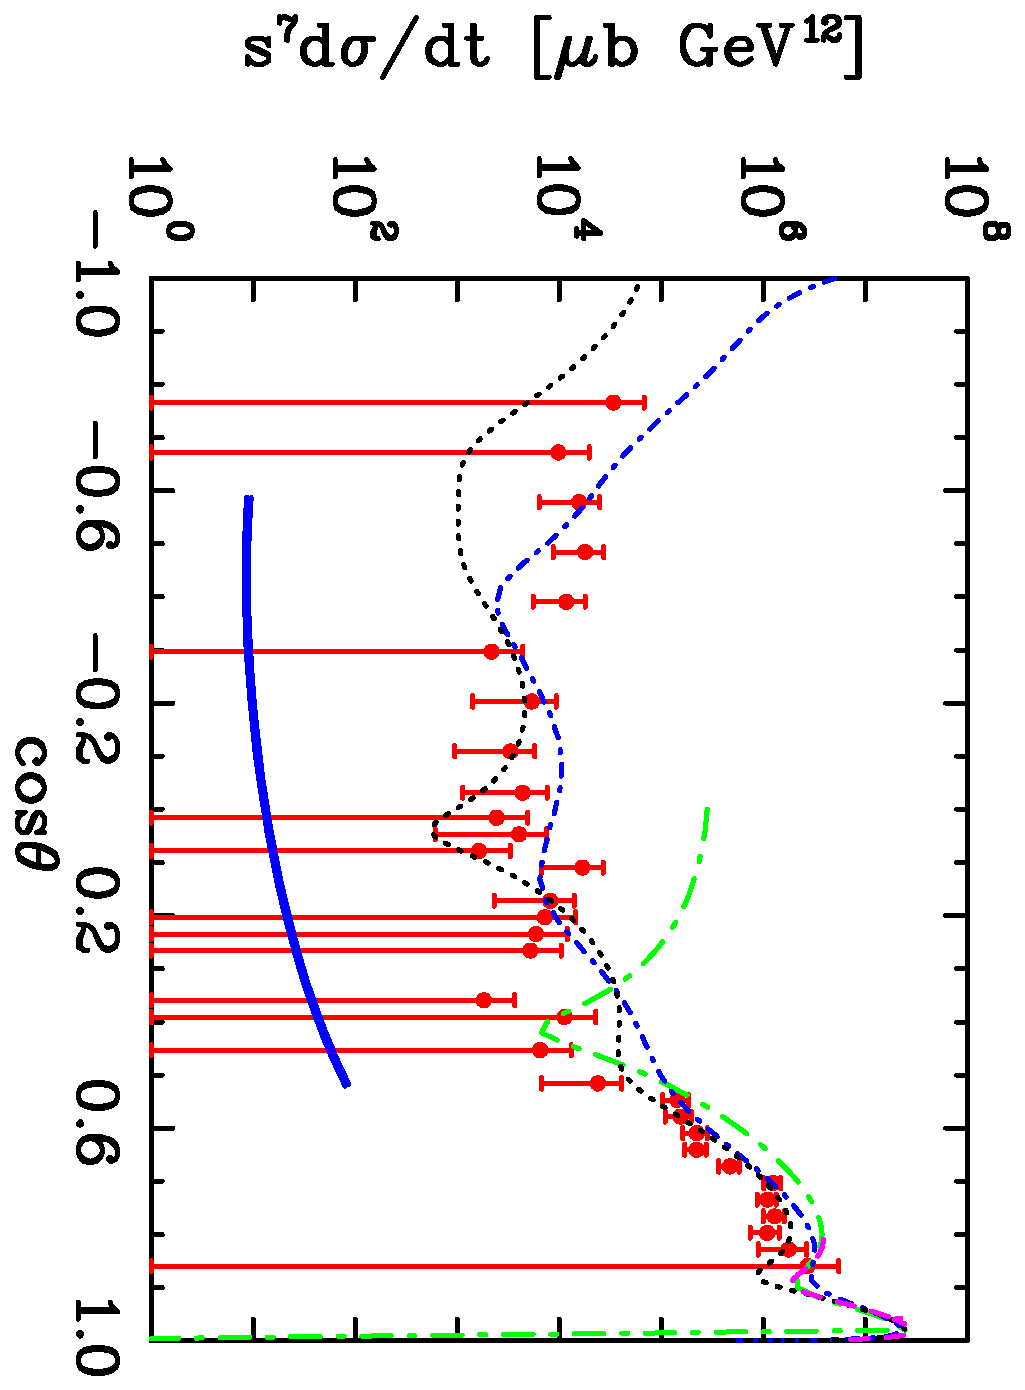
\includegraphics[width=2.5in, angle=90]{kroll.eps}}

        \caption {EPStoPDF} \label{fig:kroll}
\end{figure}
\begin{figure}
\centerline{
        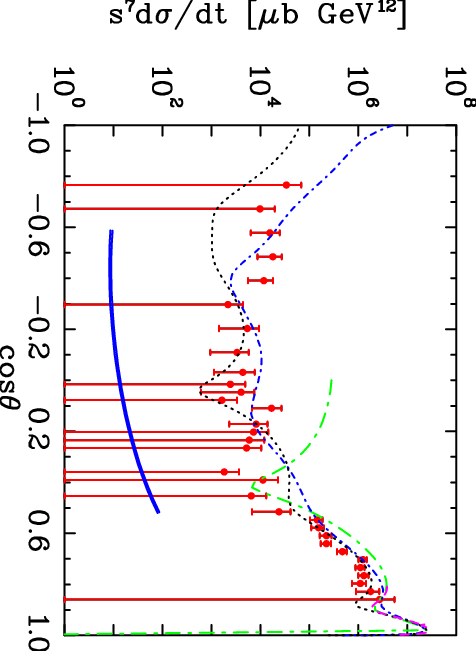
\includegraphics[width=2.5in, angle=90]{kroll.png}}

        \caption {EPStoPDF} \label{fig:krollPNG}
\end{figure}
%-----------------------------------------------------
%\FloatBarrier
%-----------------------------------------------------
%\textbf{Conclusions:} 

---
\end{document}
